%%%%%%%%%%%%%%%%%%%%%%%%%%%%%%%%%%%%%%%%%%%%%%%%%%%%%%%%%%%%%%%%%%%%%%%%%%%%%%
%
% Section file included in main project file using \input{}
%
% Assumes that LaTeX2e macros and packages defined in cg_comp.sty are
%   available
%
%%%%%%%%%%%%%%%%%%%%%%%%%%%%%%%%%%%%%%%%%%%%%%%%%%%%%%%%%%%%%%%%%%%%%%%%%%%%%%

 \section{Classical Guitar Compensation\label{sct:comp}}

 \begin{table}[htbp]
  \centering
  \caption{\label{tbl:ej45_setbacks} Predicted setbacks for the D'Addario Pro-Arte Nylon Classical Guitar Strings -- Normal Tension (EJ45) on the Alhambra 8P classical guitar.}
    \begin{tabular}{lcccc}
    \hline \hline
    String  & $\Delta S$~(mm) & $\Delta N$~(mm) \\
    \hline
    J4301 & 2.15 & -0.44 \\
    J4302 & 1.90 & -0.32 \\
    J4303 & 4.30 & -0.86 \\
    J4304 & 1.29 & -0.19 \\
    J4305 & 1.93 & -0.30 \\
    J4306 & 2.59 & -0.37 \\
    \hline \hline
    Mean & 2.36 & -0.41 \\
    \hline
    \end{tabular}%
 \end{table}%

 \begin{figure}
  \centering
  \begin{subfigure}[b]{0.45\textwidth}
   \centering
   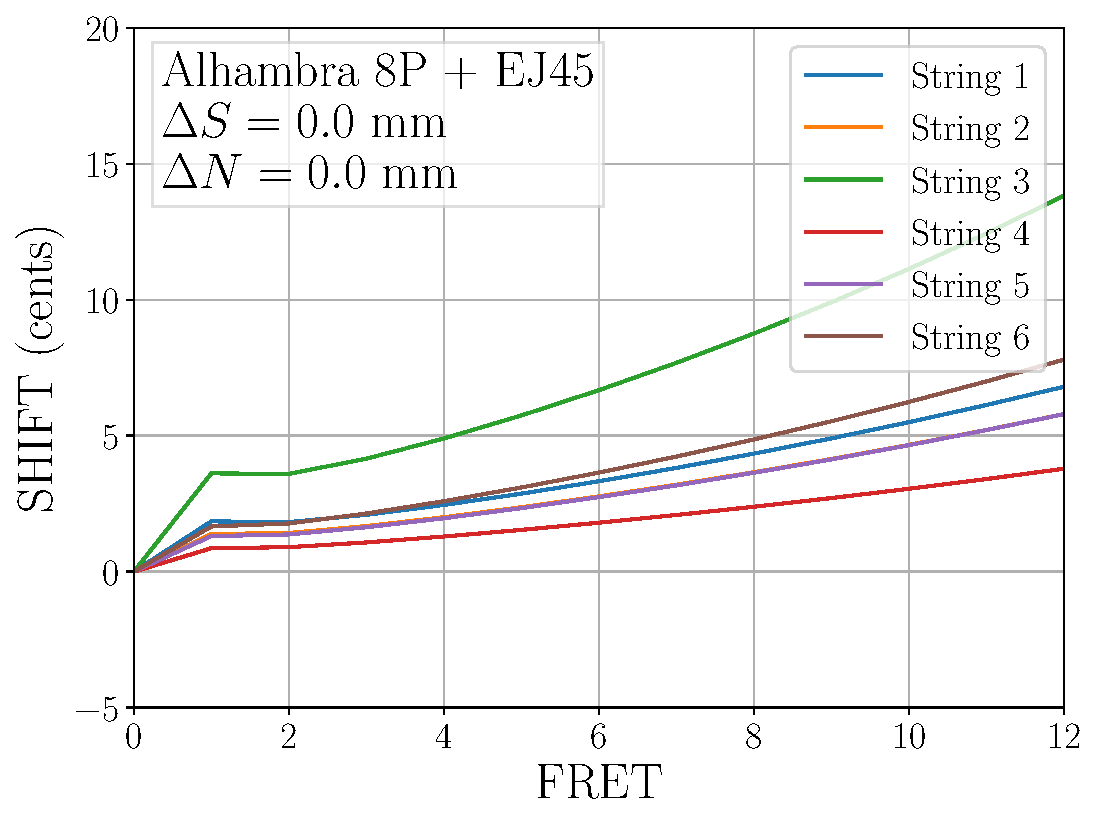
\includegraphics[width=3.25in]{figures/shift_alhambra8p_ej45_null}
   \caption{Uncompensated}
   \label{fig:shift_alhambra8p_ej45_null}
  \end{subfigure}
  \hspace{0.25in}
  \begin{subfigure}[b]{0.45\textwidth}
   \centering
   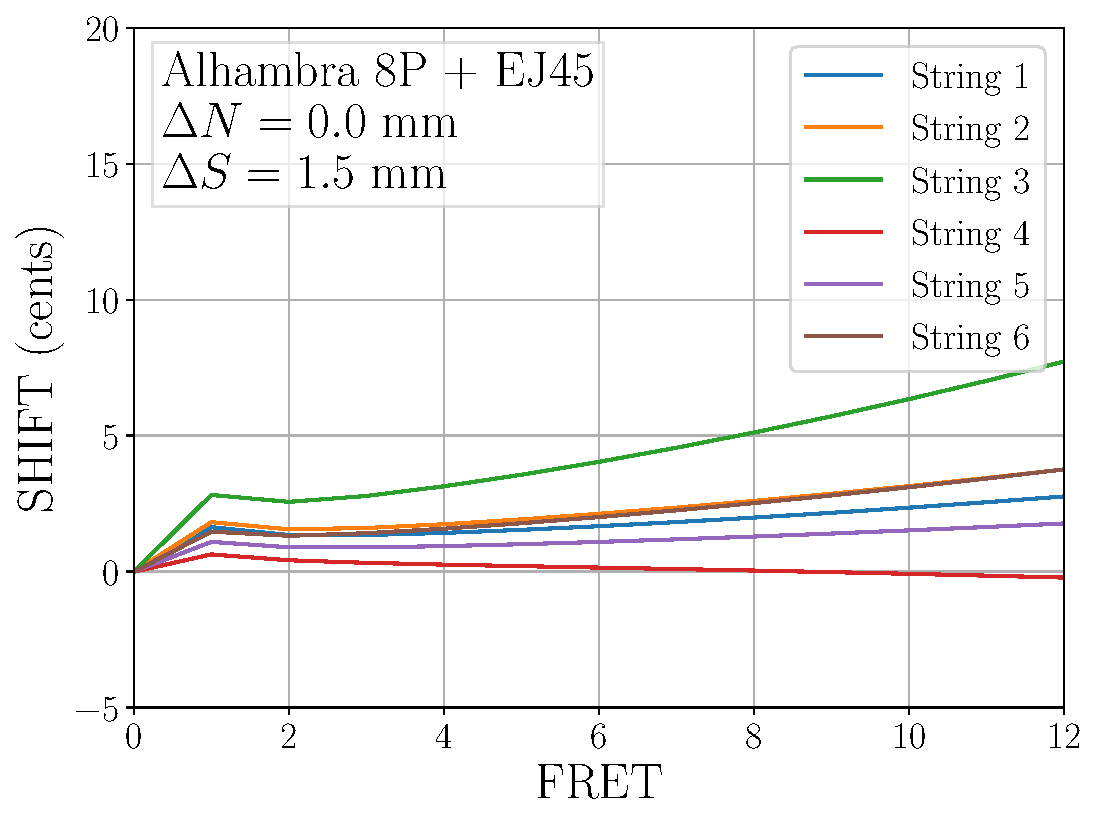
\includegraphics[width=3.25in]{figures/shift_alhambra8p_ej45_factory}
   \caption{Factory guitar}
   \label{fig:shift_alhambra8p_ej45_factory}
  \end{subfigure}
  \par\vspace{0.25in}
  \begin{subfigure}[b]{0.45\textwidth}
   \centering
   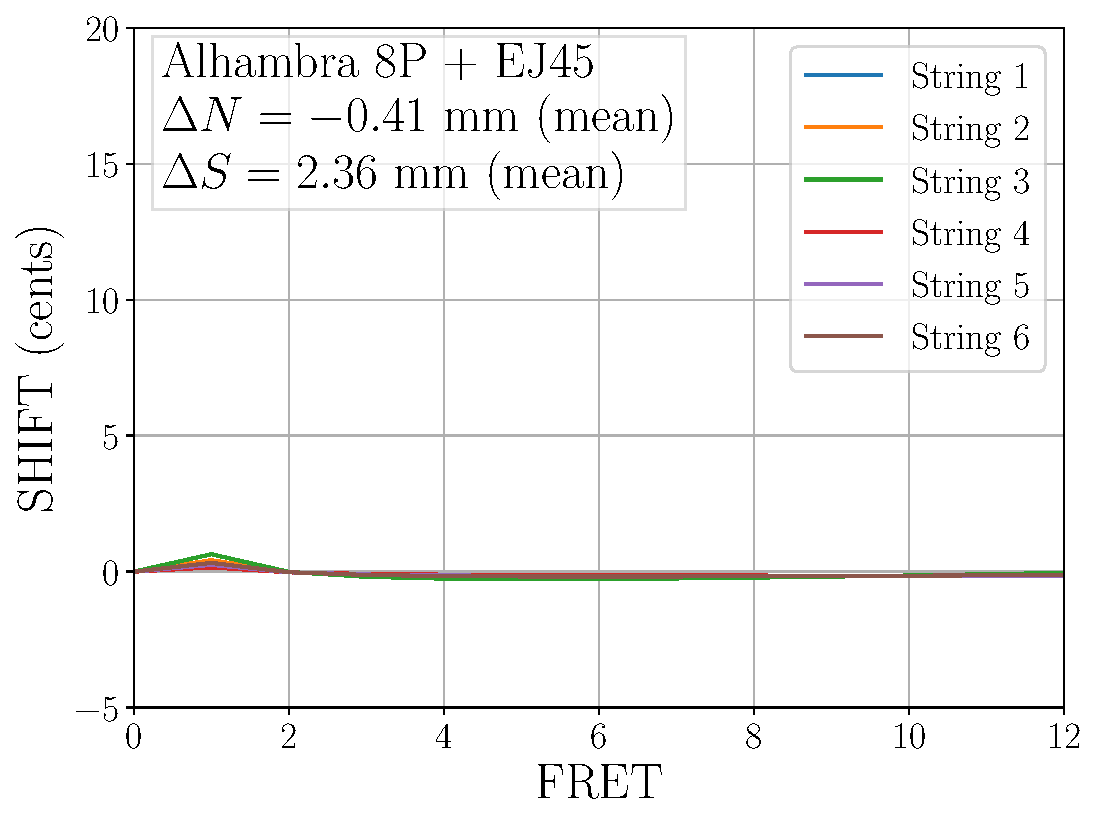
\includegraphics[width=3.25in]{figures/shift_alhambra8p_ej45_full}
   \caption{Full compensation}
   \label{fig:shift_alhambra8p_ej45_full}
  \end{subfigure}
  \hspace{0.25in}
  \begin{subfigure}[b]{0.45\textwidth}
   \centering
   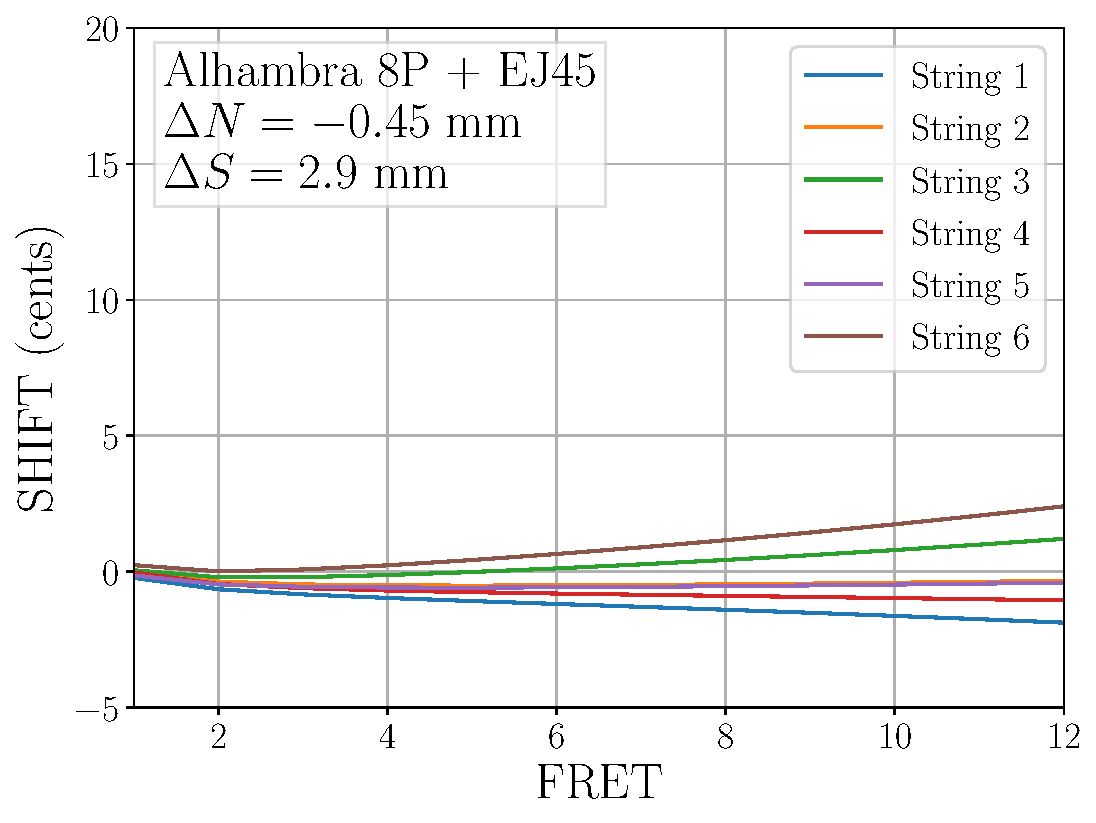
\includegraphics[width=3.25in]{figures/shift_alhambra8p_ej45_mean}
   \caption{Mean compensation}
   \label{fig:shift_alhambra8p_ej45_mean}
  \end{subfigure}
  \caption{\label{fig:compensation_alhambra8p_ej45} Frequency shift (in cents) for an Alhambra 8P guitar with D'Addario Pro-Arte Nylon Classical Guitar Strings -- Normal Tension (EJ45). Four different strategies of saddle and nut compensation are illustrated.}
 \end{figure}

